
\documentclass{beamer}
\usepackage{amsfonts,amsmath,amssymb}
\mode<presentation>
\usetheme{bbk2}
\usefonttheme[onlymath]{serif}
\usepackage{graphicx}
\usepackage{framed}
\usepackage{wasysym}
\usepackage{amsmath}
\usepackage{amsthm}
\usepackage{amsfonts}
\usepackage{mathtools} 

\theoremstyle{definition}

\newtheorem{conjecture}{Conjecture:}
\newenvironment{hproof}{
  \renewcommand{\proofname}{Sketch Proof}\proof}{\endproof}
\numberwithin{theorem}{section}






\begin{document}

\title[Persistent Homology]{Persistent Homology of Maps on Filtrations of Simplicial Complexes}
\author{O. Turnbull}
\institute[Birkbeck College]{Department of Economics, Mathematics and Statistics\\
Birkbeck, University of London\\ \vspace{0.7cm}

\includegraphics[width=2cm]{bbklogo.jpg}}
\date{December 2020}
\begin{frame}\titlepage
\end{frame}

\begin{frame}
\frametitle{Introduction}
\begin{block}{Intro to Algebraic Topology}
Algebraic Topology can be described as the application of algebraic techniques to solve topological problems
\begin{itemize}
\item{Homotopy Equivalence}
\item{Simplicial Complexes}
\item{Homology}
\end{itemize}
\end{block}
\end{frame}

\begin{frame}
\frametitle{A Quick Refresher}
\begin{block}{Topological Spaces}
\begin{definition}
A topological space $(X, \tau )$ is a set $X$ coupled with a collection of sets $\tau \subset 2^{X}$ satisfying the following axioms:

\begin{enumerate}
\item{$\varnothing \in \tau$}
\item{$X \in \tau$}
\item{$\forall U_1, U_2 \in \tau, U_1 \cap U_2 \in \tau$}
\item{ If $\forall i \in I \; U_i \in \tau $, $I$ some indexing set, then $\bigcup_{i \in I} U_i \in \tau$}
\end{enumerate}
\end{definition}
The elements of $\tau$ are called open sets in $X$.
\end{block}
\end{frame}

\begin{frame}
\frametitle{More Refreshments}
\begin{block}{Topological Maps}
\begin{definition}
A continuous map is an $f:X\rightarrow Y$ such that whenever $V$ is open in $Y$, $f^{-1}(V)$ is open in $X$.
\end{definition}
\begin{definition}
A function is a homeomorphism if it is bijective and both it and its inverse are continuous. If two topological spaces permit a homeomorphism, they are homeomorphic.
\end{definition}
\end{block}
\end{frame}
\begin{frame}
\begin{block}{Topological Maps}
\begin{definition}
Two functions $f: X\rightarrow Y$ and $g: X \rightarrow Y$ ($X$ and $Y$ topological spaces) are said to be homotopic to one another by a homotopy $H: X \times [0,1] \rightarrow Y$ if $H(x,0) = f(x)$, $H(x,1) = g(x)$ and H is continuous.\newline
Two spaces $X$, $Y$ are said to be Homotopy equivalent if there exist maps $f$, $g$ such that $f \circ g$ is homotopic to the identity on $Y$, and $g \circ f$ homotopic to the identity on $X$.
\end{definition}



\end{block}
\end{frame}




\begin{frame}
\small
\frametitle{Simplicial Complexes}
\begin{block}{Hyper-dimensional Triangles}
\begin{definition}
A $k$- \textbf{simplex} is the subset of $\mathbb{R}^n$ defined by
\scriptsize
$$\{ a_0v_0+ a_1v_1+ \hdots + a_kv_k \; | \; a_0 + a_k + \hdots + a_k = 1 \; \textrm{and} \; a_i \geq 0 \;\textrm{for} \;i = 1, 2, \hdots, k \}$$
\small

\end{definition}
The convex hull of any subset of the $n+1$ points that define a simplex is called a \textit{face} of that simplex, and is itself a simplex.
These can then be \textit{glued} together in a certain sense to form a simplicial complex:
\begin{definition}
A \textbf{simplicial complex} is a collection of simplicies $K$ such that 
\begin{itemize}
\item{Every face of a simplex in $K$ is a member of $K$}
\item{$\forall \sigma_1, \sigma_2 \in K, \; \sigma_1 \cap \sigma_2 = \varnothing$ or $\eta$ such that $\eta$ is a face of both $\sigma_1$ and $\sigma_2$}
\end{itemize}
\end{definition}
\end{block}
\end{frame}

\begin{frame}[t]
\frametitle{Simplicial Homology}

\begin{block}{Chain complexes}
\scriptsize
We can define a free abelian group on a simplicial complex by giving each member $k$-simplex an orientation and considering the set of simplicial $k$-chains $\sum^{N}_{i=1} = c_i\sigma_i$, where each $c_i$ an integer and $\sigma_i = (v_0, \hdots, v_k)$ a generator associated each a $k$-simplex, appropriately oriented. Call this group $C_k$ 
\end{block}
\begin{columns}[t]
\begin{column}{0.4\textwidth}
\begin{block}{The boundary homomorphism}
\tiny
Let $X$ be a simplicial complex and $\sigma$ be an oriented $k$-simplex that is a face of $X$. The boundary map $\partial _k: C_k \rightarrow C_{k-1}$ is defined by the homomorphism $$\partial_k(\sigma) = \Sigma_{i=0}^k (-1)^i (v_0, \hdots, \hat{v_i}, \hdots, v_k)$$ 
The $k$-th homology group is thence $$H_k(X) = \frac{\textrm{ker}(\partial_{k})}{\textrm{im}(\partial_{k+1})}$$ 
\end{block}
\end{column}
\begin{column}{0.4\textwidth}
	\begin{figure}
		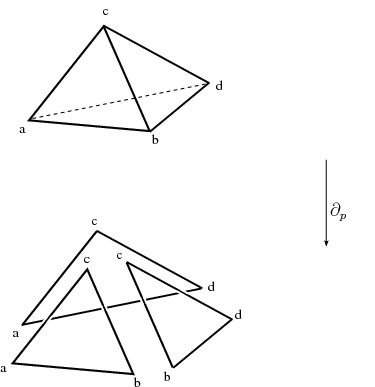
\includegraphics[width = 4cm]{img670.png}
	\end{figure}
\end{column}
\end{columns}
\end{frame}



\begin{frame}
\frametitle{Triangulation}
\begin{block}{Topological skeletons}
A \textbf{triangulation} of a Topological Space $X$ is a simplicial complex $K$, with a homeomorphism $h : X \rightarrow K$. 
\end{block}

\end{frame}

\begin{frame}{Visuals}
\vspace{0.1cm}
\begin{columns}

	\begin{column}{0.3\textwidth}
		\begin{figure}
		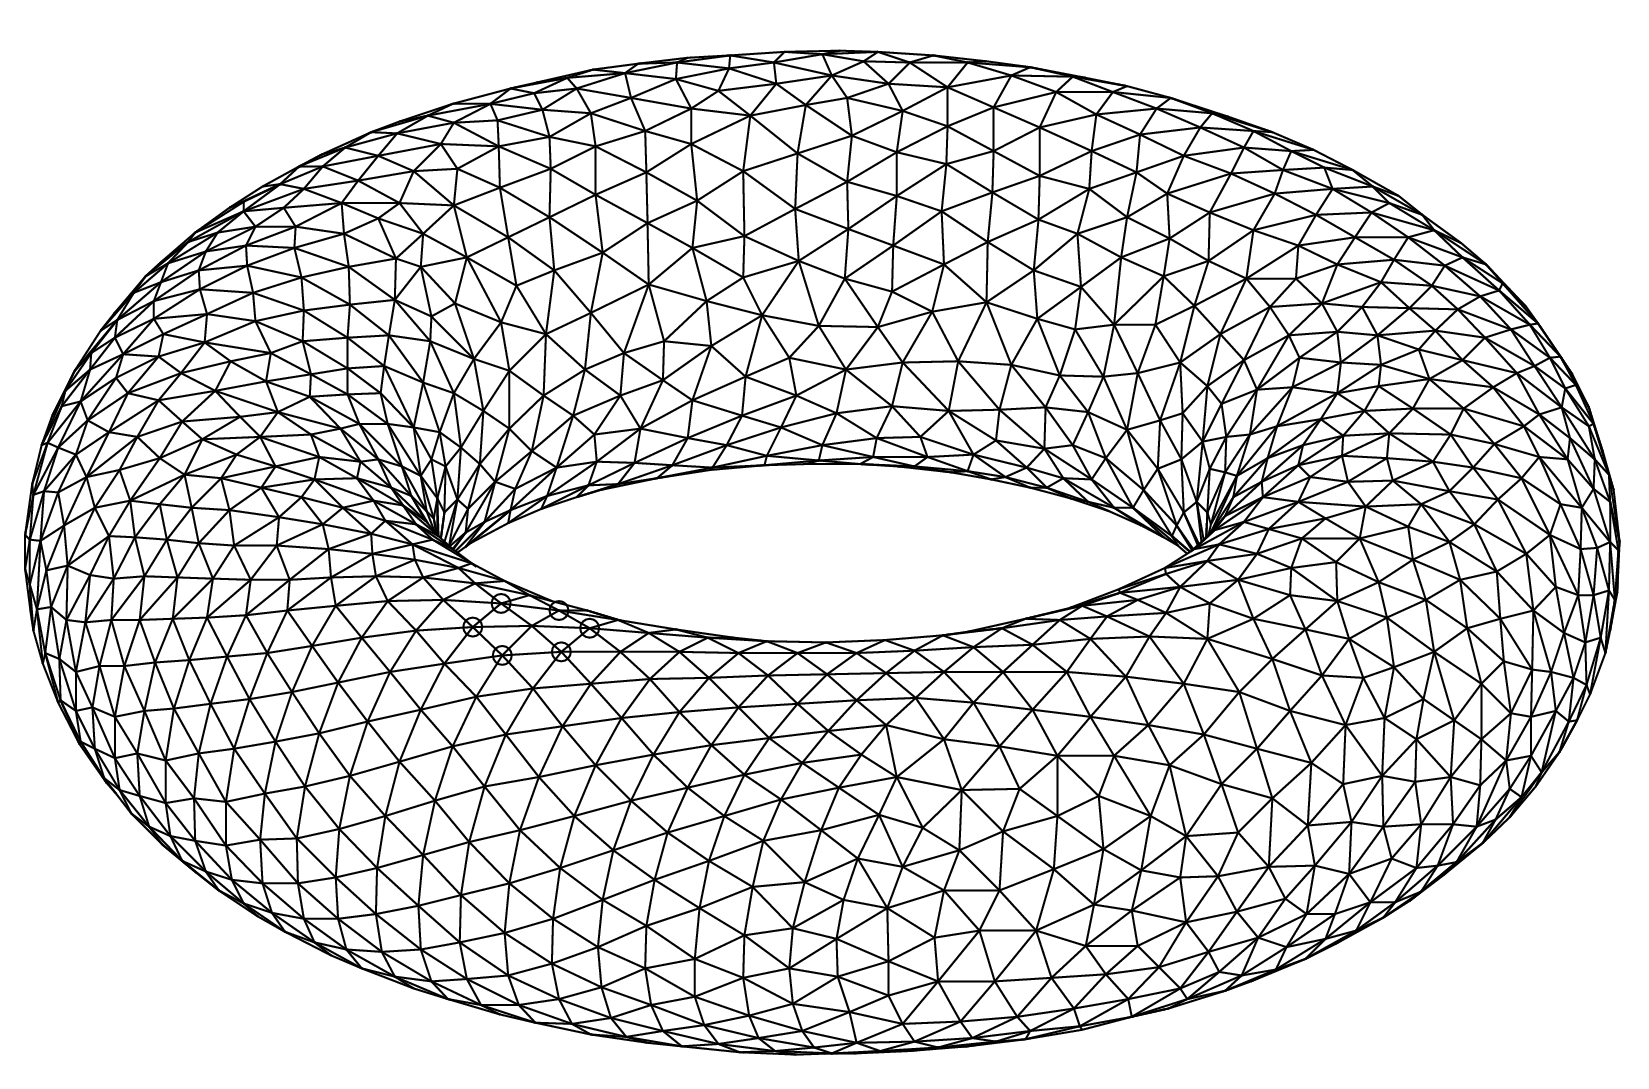
\includegraphics[width = 5cm]{Torus-triang.png}
		\tiny
		%\caption*{\tiny Mathematician G. H. Hardy}
	\end{figure}
	\end{column}
	\begin{column}{0.6\textwidth}
		\begin{figure}
		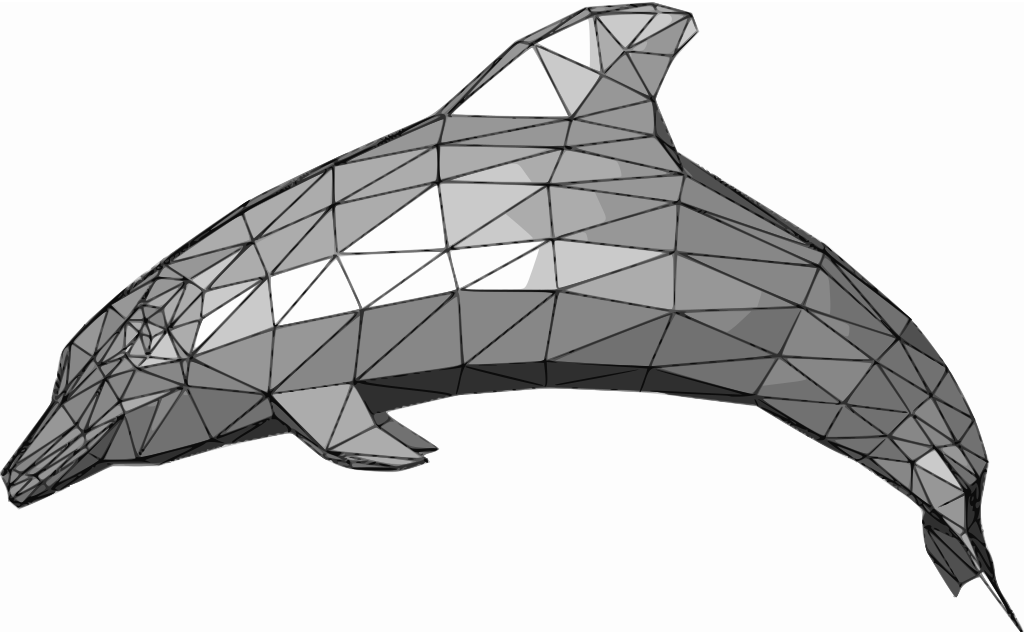
\includegraphics[width = 5cm]{Dolphin_triangle_mesh.png}
		\tiny
		%\caption*{\tiny Mathematician G. H. Hardy}
		\end{figure}

	\end{column}
\end{columns}
\end{frame}


\begin{frame}
\frametitle{Persistence}
\begin{block}{Maps on simplicial complexes}
Let $K$ be a simplicial complex and let $f:K\rightarrow\mathbb{R}$ be a nondecreasing map on faces i.e. $f(\tau)\leq f(\sigma)$ whenever $\tau$ is a face of $\sigma$. Then for every $a\in\mathbb{R}$, the sublevel set $K(a) = f^{-1}((-\infty,a])$ is a subcomplex of $K$, and this induces an ordering on sublevel complexes defining a \textit{filtration} $$\varnothing = K_0 \subset K_1 \subset \cdots \subset K_n = K$$ These furthermore induce homomorphisms on these homology groups $f^{i,j}_p: H_p(K_i)\rightarrow H_p(K_j)$, the images of these maps given a $p$ are called the $p^{\textrm{th}}$ persistent homology groups.
\end{block}
\end{frame}

\begin{frame}
\frametitle{Persistence (cont.)}
	\begin{block}{Birth and Death and Barcodes}
	\begin{itemize}
		\item{In the aforementioned ordering of sublevel subcomplexes, we have $K_i = K(a_i) = f^{-1}((-\infty, a_i])$ i.e $a_n=\infty$ and so each of these homology groups $\mathrm{im}f^{i,j}_p$ describes the classes 'born' at 'time' $a_i$ and 'persisting' (i.e. still alive) at 'time' $a_j$.} 
		\item{The ranks of these groups, called the \textbf{persistent Betti numbers} of $f$, $\beta^{i,j}_p = \mathrm{rank}\; \mathrm{im}f_p^{i,j}$ will then give you the number of generators of the homology groups, and thus an understanding of some topological features of $f^{-1}((-\infty, t])$ for $t\in (a_i, a_j)$} 
		\item{In this sense, you can plot the multiplicity of these Betti numbers over the range of $f$ to get a sense of how long these features 'last'}
	\end{itemize}
	\end{block}
\end{frame}
\begin{frame}[t]
\begin{figure}
		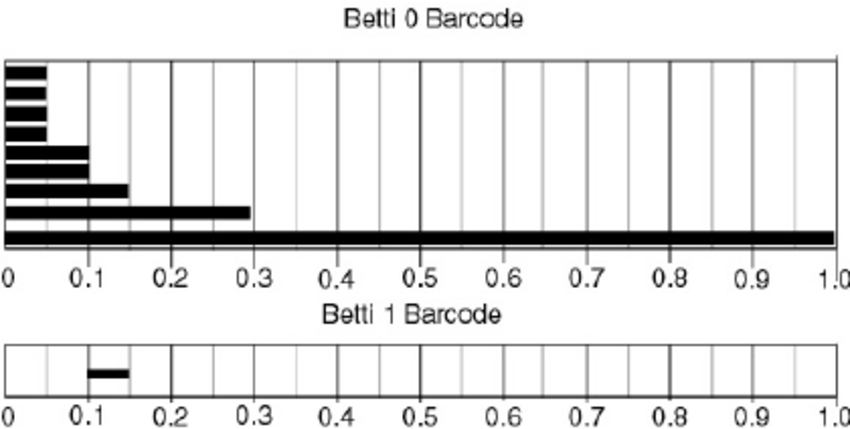
\includegraphics[width = 6cm]{Betti-0-and-Betti-1-persistence-barcode-of-S-50-the-output-from-the-noisy-point-P-in.png}
		\tiny
		\caption{an example of a persistence barcode diagram}
		\end{figure}
\begin{block}{Stability}
\scriptsize
	Luckily, these kind of diagrams are stable in a precise sense: 
	\begin{itemize}
		\item A natural metric on the space of persistence diagrams is $$W(X,Y) := \underset{\varphi: X \rightarrow Y}{\mathrm{inf}} \underset{x \in X}{\mathrm{sup}} \| x - \varphi (x) \|  $$
		\item This is called the \textbf{Bottleneck Distance}, and it can be shown that a small perturbation in the input filtration leads to a small perturbation in this metric. 
	\end{itemize}
\end{block}
\end{frame}

\begin{frame}
\frametitle{Applications}
\begin{block}{Why do we care? Topological Data Analysis}

\end{block}
\begin{columns}[t]
	\begin{column}{0.4\textwidth}
	\begin{figure}
	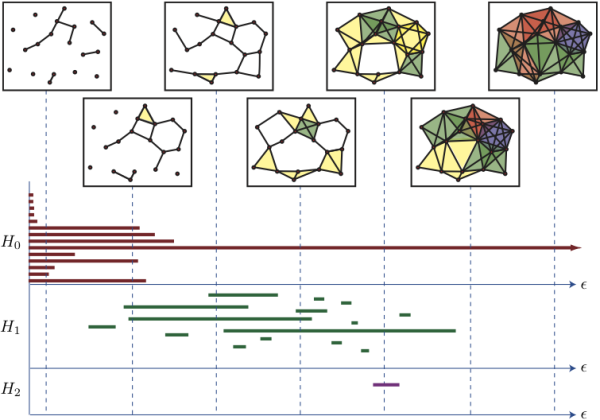
\includegraphics[width = 4cm]{barcode-crop.png}
		
		%\caption*{\tiny Mathematician G. H. Hardy}
		\end{figure}
		\begin{figure}
	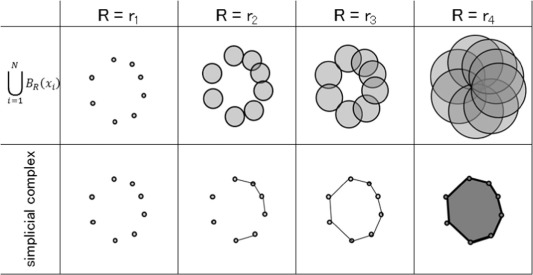
\includegraphics[width = 4cm]{persist.jpg}
		\tiny
		%\caption*{\tiny Mathematician G. H. Hardy}
		\end{figure}
	\end{column}
	\begin{column}{0.4\textwidth}
	\begin{block}{Distance Functions}
	\scriptsize
		We can construct one such face-nondecreasing function by considering the simplicial complex formed when joining $n$ points in a point cloud together with an $n$-simplex when their respective balls of radius $r$ intersect, then $f(\sigma) = r$  gives us the kind of function we need to do persistent homology. 
		\begin{itemize}
			\item{helps us find topological features in data and how 'strong' they are.}
		\end{itemize}
	\end{block}
	\end{column}
\end{columns}
\end{frame}

\begin{frame}
\frametitle{Further Research}
\begin{block}{Higher dimensions...}
What if we have...
\begin{itemize}
	\item more than one face-nondecreasing function on our simplicial complex?
	\item want to summarise properties of one function through the homology of another (i.e. how persistent homology might evolve in time)
	\item different kinds of maps from simplicial complexes to spaces such as probability measures, other kinds of point cloud distance functions, etc.
\end{itemize}
In short, what other features can we infer about functions from their persistent homology, and what other features of functions can we summarise with topological methods?
\end{block}
\end{frame}

\end{document}
